\documentclass[tikz,border=5pt]{standalone}

\usepackage{tikz}
\usetikzlibrary{positioning}

\begin{document}

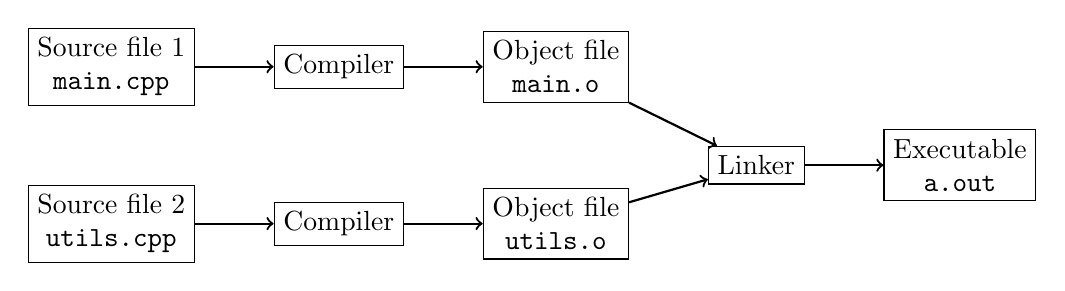
\begin{tikzpicture}[
    node distance=1cm,
    every node/.style={draw, rectangle, align=center, minimum height=0cm},
    arrow/.style={->, thick}
]

% Source files
\node (s1) {Source file 1\\ \texttt{main.cpp}};
\node (s2) [below=of s1] {Source file 2\\ \texttt{utils.cpp}};

% Compiler
\node (c1) [right=of s1, xshift=0cm] {Compiler};
\node (c2) [right=of s2, xshift=0cm] {Compiler};

% Object files
\node (o1) [right=of c1, xshift=0cm] {Object file\\ \texttt{main.o}};
\node (o2) [right=of c2, xshift=0cm] {Object file\\ \texttt{utils.o}};

% Linker
\node (l) [right=of o1, yshift=-1.25cm, xshift=0cm] {Linker};

% Executable
\node (e) [right=of l, xshift=0cm] {Executable\\ \texttt{a.out}};

% Arrows
\draw[arrow] (s1) -- (c1);
\draw[arrow] (c1) -- (o1);

\draw[arrow] (s2) -- (c2);
\draw[arrow] (c2) -- (o2);

\draw[arrow] (o1) -- (l);
\draw[arrow] (o2) -- (l);

\draw[arrow] (l) -- (e);

\end{tikzpicture}

\end{document}
